\section {Функция Швефеля}
\label{TestFunctions:section:HML_TestFunction_Schwefel}
\subsection {Описание функции}

\begin{tabularwide}
\textbf{Идентификатор:} & HML\_TestFunction\_Schwefel. \\
\textbf{Наименование:} & Функция Швефеля. \\
\textbf{Тип:} & Задача вещественной оптимизации. \\
\end{tabularwide}

\textbf{Формула} (целевая функция):
\begin{equation}
\label{TestFunctions:eq:HML_TestFunction_Schwefel}
f\left( \bar{x}\right) = 418.9829 n-\sum_{i=1}^{n}\left( \bar{x}_i\sin\left( \sqrt{\left| \bar{x}_i\right|}\right)  \right), \text{ где}
\end{equation}
\indent $\bar{x}\in X$, $\bar{x}_j\in \left[ Left_j; Right_j\right] $, $Left_j=-500$, $Right_j=500$, $j=\overline{1,n}$.

\begin{tabularwide}
\textbf{Обозначение:} &\specialcell{$\bar{x}$ --- вещественный вектор;\\$n$ --- размерность вещественного вектора.}  \\
\textbf{Решаемая задача оптимизации:} & $\bar{x}_{min}= \arg \min_{\bar{x}\in X} f\left( \bar{x}\right)$.   \\
\textbf{Точка минимума:} & $\bar{x}_{min}={\left( 420.968746,420.968746,\ldots,420.968746\right)}^\mathrm{T} $, то есть $\left(\bar{x}_{min} \right)_j=420.968746$ ($j=\overline{1,n}$).    \\
\textbf{Минимум функции:} & \specialcell{$f\left(\bar{x}_{min} \right) =0.0000255$, если $ n=2 $.\\$f\left(\bar{x}_{min} \right) =0.000127276$, если $ n=10$. \\То есть для каждого значения $ n$ надо пересчитывать\\ значение глобального минимума.}   \\
\textbf{График:} & Рисунок \ref{TestFunctions:img:HML_TestFunction_Schwefele} нас \pageref{TestFunctions:img:HML_TestFunction_Schwefele} стр.   \\
\end{tabularwide}

\begin{figure} [h] 
  \center
  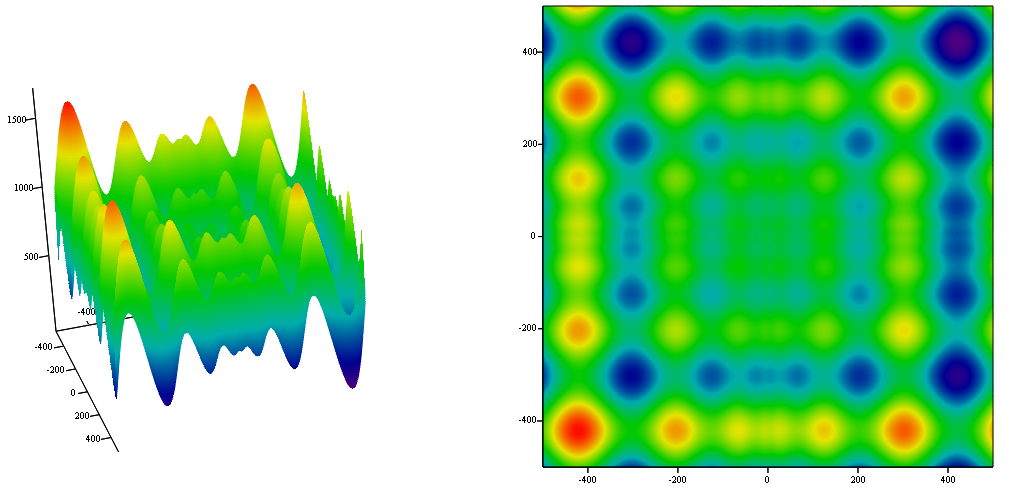
\includegraphics [scale=0.5] {HML_TestFunction_Schwefel}
  \caption{Функция Швефеля} 
  \label{TestFunctions:img:HML_TestFunction_Schwefele}  
\end{figure}

\subsection {Параметры для алгоритмов оптимизации}

\begin{tabularwide}
\textbf{Точность вычислений:} & $\varepsilon=2.5$. \\
\textbf{Число интервалов, на которые предполагается разбивать каждую компоненту вектора $\bar{x}$ в пределах своего изменения} (для алгоритмов дискретной оптимизации) : & $NumberOfParts_j=4095$ ($j=\overline{1,n}$). \\
\textbf{Для этого длина бинарной строки для $x_j$ координаты равна} (для алгоритмов бинарной оптимизации) : & $\left( k_2\right)_j=12$ ($j=\overline{1,n}$). \\
\end{tabularwide}

\textbf{Замечание:}  $NumberOfParts_j$ выбирается как минимальное число, удовлетворяющее соотношению:
\begin{equation*}
NumberOfParts_j=2^{\left( k_2\right)_j }-1\geq\dfrac{10\left( Right_j-Left_j\right) }{\varepsilon},\text{где } \left( k_2\right)_j \in \mathbb{N}, \left( j=\overline{1,n}\right).
\end{equation*}

\subsection {Основная задача и подзадачи}

\begin{tabularwide}
\textbf{Изменяемый параметр: } & $n$ --- размерность вещественного вектора. \\
\textbf{Значение в основной задаче:} & $n=2$.\\
\textbf{Подзадача №2:} & $n=3$.\\
\textbf{Подзадача №3:} & $n=4$.\\
\textbf{Подзадача №4:} & $n=5$.\\
\textbf{Подзадача №5:} & $n=10$.\\
\textbf{Подзадача №6:} & $n=20$.\\
\textbf{Подзадача №7:} & $n=30$.\\
\end{tabularwide}

\subsection {Нахождение ошибки оптимизации}

Пусть в результате работы алгоритма оптимизации за $N$ запусков мы нашли решения $\bar{x}_{submin}^k$ со значениями целевой функции $f\left( \bar{x}_{submin}^k\right) $ соответственно ($k=\overline{1,N}$). Используем три вида ошибок:

\textbf{Надёжность: }
\begin{equation*}
R = \dfrac{\sum_{k=1}^{N}S\left( \bar{x}_{submin}^k \right) }{N}, \text{ где}
\end{equation*}
\begin{equation*}
S\left( \bar{x}_{submin}^k \right)=\left\lbrace \begin{aligned} 1,& \text{ если } \left| \left( \bar{x}_{submin}^k \right)_j-\left( \bar{x}_{min} \right)_j\right|<\varepsilon, j=\overline{1,n};   \\ 0,& \text{ иначе}. \end{aligned}\right.
\end{equation*}

\textbf{Ошибка по входным параметрам:}
\begin{equation*}
E_x = \dfrac{\sum_{k=1}^{N} \left( \frac{\sqrt{\sum_{j=1}^{n}{\left( \left( \bar{x}_{submin}^k \right)_j-\left( \bar{x}_{min} \right)_j \right)}^2 }}{n} \right)  }{N}.
\end{equation*}

\textbf{Ошибка по значениям целевой функции: }
\begin{equation*}
E_f = \dfrac{\sum_{k=1}^{N} \left| f\left( \bar{x}_{submin}^k \right)-f\left( \bar{x}_{min} \right) \right|  }{N}.
\end{equation*}

\subsection {Свойства задачи}
\begin{tabularwide}
\textbf{Условной или безусловной оптимизации: } & Задача безусловной оптимизации. \\
\textbf{Одномерной или многомерной оптимизации: } & Многомерной: $ n $. \\
\textbf{Функция унимодальная или многоэкстремальная: } & Функция многоэкстремальная. \\
\textbf{Функция стохастическая или нет: } & Функция не стохастическая. \\
\textbf{Особенности: } & Для каждого значения $ n$ надо пересчитывать значение глобального минимума. \\
\end{tabularwide}

\subsection {Реализация}

Реализация функции взята из библиотеки HarrixMathLibrary в разделе <<Тестовые функции для оптимизации>>, которую можно найти по адресу \href{https://github.com/Harrix/HarrixMathLibrary} {https://github.com/Harrix/HarrixMathLibrary}.

\begin{lstlisting}[caption=Код функции HML\_TestFunction\_Schwefel]
double double HML_TestFunction_Schwefel(double *x, int VHML_N)
{
/*
Функция многих переменных: функция Швефеля.
Тестовая функция вещественной оптимизации.
Входные параметры:
 x - указатель на исходный массив;
 VHML_N - размер массива x.
Возвращаемое значение:
 Значение тестовой функции в точке x.
*/
double VHML_Result=418.9829*VHML_N;

for (int i=0;i<VHML_N;i++)
    VHML_Result -= x[i]*sin(sqrt(fabs(x[i])));

return VHML_Result;
}
\end{lstlisting}

\subsection {Ссылки}

Данная функция приводится в следующих источниках:

\begin{enumerate}
\item \cite[стр. 9]{web:1207.4318} ---  \href{http://arxiv.org/pdf/1207.4318v1.pdf}{Empirical review of standard benchmark functions using evolutionary global optimization}.
\item \cite{web:www.cs.cmu.edu:BenchmarkProblems} ---  \href{http://www.cs.cmu.edu/afs/cs/project/jair/pub/volume24/ortizboyer05a-html/node6.html}{Benchmark Problems}.
\end{enumerate}

Обратите внимание, что в англоязычном секторе часто данная функция дается с обозначением глобального минимума в точке $\left(\bar{x}_{min} \right)_j=1$ ($j=\overline{1,n}$), $f\left(\bar{x}_{min} \right) =0$ (например, \cite{web:www.sfu.ca:SchwefelFunction}, \cite{web:www-optima.amp.i.kyoto-u.ac.jp:SchwefelFunction}). Это не правильно: $f\left(\begin{matrix}
1 \\ 1
\end{matrix} \right) =836.28286$. Скорее всего в каком-то источнике вначале допустили ошибку, и она стала копироваться в остальные.

В некоторых источниках (например, \cite{web:www.pg.gda.pl:Schwefelsfunction7}, \cite[стр. 7]{web:GEATbxExamples}) в формуле тестовой функции присутствует только второе слагаемое, а глобальный минимум определяется как $ 418.9829 n $. Это неправильно, так как хоть два слагаемых похожи друг на друга (\ref{TestFunctions:eq:HML_TestFunction_Schwefel}), но они не дают строгий ноль в сумме, и при увеличении размерности различие между ними увеличивается.